\documentclass{ctexbeamer}
% \documentclass{beamer}
\usetheme{Warsaw}
\usepackage{graphicx}
\usepackage{beamerbasetitle}
\usepackage{listing}
\usefonttheme[onlymath]{serif}
\usepackage{hyperref}
\hypersetup{
  colorlinks,
  allcolors=.,
  urlcolor=blue,
}
\graphicspath{ {./images/} }
\usepackage{multicol}
\definecolor{PKUblack}{rgb}{0, 0, 0} % UBC Blue (primary)
\definecolor{PKUred}{HTML}{b23333} % UBC Grey (secondary)

\setbeamercolor{palette primary}{bg=PKUred,fg=white}
\setbeamercolor{palette secondary}{bg=PKUblack,fg=white}
\setbeamercolor{palette tertiary}{bg=PKUblack,fg=white}
\setbeamercolor{palette quaternary}{bg=PKUblack,fg=white}
\setbeamercolor{structure}{fg=PKUred} % itemize, enumerate, etc
\setbeamercolor{section in toc}{fg=PKUred} % TOC sections

% Override palette coloring with secondary
\setbeamercolor{subsection in head/foot}{bg=PKUred,fg=white}

\title{P, NP and NP-complete}
\author{方嘉聪 2200017849}
\institute{北京大学}
\date{\today}
\begin{document}
    % \large
    \begin{frame}
        \titlepage
    \end{frame}

    \AtBeginSection[]
    {
        \begin{frame}<beamer>
            \frametitle{目录}
            \tableofcontents[currentsection]
        \end{frame}
    }
    \section{Definition}
\subsection{Turing Machine}
\begin{frame}
    \frametitle{Deterministic Turing Machine}
\begin{definition}[Deterministic Turing Machine]
    A $k$-tape TM is a 7-tuple $(Q, \Sigma, \Gamma, \delta, q_0, q_{accept}, q_{reject})$:
    \begin{itemize}
        \item $Q$ sets of states, $\Sigma$ input alphabet, $\Gamma$ tape alphabet
        \item $\delta: Q\times \Gamma^k \rightarrow Q\times \Gamma^k\times \{L,S,R\}^k$ transition function
        \item $q_0$ initial state, $q_{accept}$ accepting state, $q_{reject}$ rejecting state
    \end{itemize}
\end{definition}
\pause
\begin{definition}[Computation of a TM]
    A TM $M$ accepts input $w$ if a sequence of configurations $C_1, C_2, \ldots, C_k$ exists such that:
    \begin{itemize}
        \item $C_1$ is the start configuration of $M$ on input $w$;
        \item each $C_i$ yeilds $C_{i+1}$ by applying $\delta$;
        \item $C_k$ is an accepting configuration.
    \end{itemize}
\end{definition}
\end{frame}

\begin{frame}
    \frametitle{Universal Turing Machine}
\begin{definition}[Universal Turing Machine]
    A TM $U$ is a universal TM if it can \textbf{simulate} any TM $M$.
\end{definition}

\begin{theorem}
    存在一个通用图灵机$U$,对于任意图灵机$M$和输入$x$, $U$能够在$O(T\log T)$时间内输出$M(x)$.
\end{theorem}
形式化书写和证明这里略去.
\end{frame}

\begin{frame}
    \frametitle{Nondeterministic Turing Machine}
\begin{definition}[Nondeterministic Turing Machine]
    A $k$-tape NTM is a 7-tuple $(Q, \Sigma, \Gamma, \delta, q_0, q_{accept}, q_{reject})$:
    \begin{itemize}
        \item $Q$ sets of states, $\Sigma$ input alphabet, $\Gamma$ tape alphabet
        \item $\delta: Q\times \Gamma^k \rightarrow 2^{Q\times \Gamma^k\times \{L,S,R\}^k}$ transition function
        \item $q_0$ initial state, $q_{accept}$ accepting state, $q_{reject}$ rejecting state
    \end{itemize}
\end{definition}
\pause
\begin{itemize}
    \item 直觉上理解, NTM在每一步都可以选择多种可能的转移, 但只要有一种转移路径能够接受, 则NTM接受输入.
    \item 运行时间: 对于函数$T: N\rightarrow N$, 一个NDTM $N$的运行时间是$T(n)$的, 如果对于任意输入长度为$n$的输入, $N$的所有分支都在$T(n)$步内停机.
\end{itemize}
\end{frame}
\subsection{P and NP}
\begin{frame}
    \frametitle{Class P}
    \begin{definition}[Class DTIME]
        设函数$T: N\rightarrow N$, 那么$\text{DTIME}(T(n))$为所有可以在$O(T(n))$时间内被确定性图灵机判定(decided)的语言的集合.
    \end{definition}
    \begin{definition}[Class P]
        $\text{P} = \bigcup_{c\in N} \text{DTIME}(n^c)$
    \end{definition}
\end{frame}

\begin{frame}
    \frametitle{Class NP}
    \begin{definition}[Class NTIME]
        设函数$T: N\rightarrow N$, 那么$\text{NTIME}(T(n))$为所有可以在$O(T(n))$时间内被非确定性图灵机判定(decided)的语言的集合.
    \end{definition}
    \begin{definition}[Class NP]
        $\text{NP} = \bigcup_{c\in N} \text{NTIME}(n^c)$
    \end{definition}
\end{frame}
\begin{frame}
    \frametitle{Class NP(Cont.)}
    \begin{definition}[Another Definition of NP]
        称一个语言$L \in $NP, 如果存在一个多项式函数$P: N \rightarrow N$, 和多项式时间的确定性图灵机$M$, 使得:
        \begin{align*}
            \forall x \in \{0,1\}^*, ~x\in L \iff \exists u \in \{0,1\}^{P(|x|)}, ~s.t.~ M(x,u) = 1
        \end{align*}
        把$u$称为$x$的证书(certificate), $M$称为$L$的验证机(verifier).
    \end{definition}
    \pause
    \begin{itemize}
        \item 直觉上理解, NP包括了所有可以在多项式时间内验证一个解是否正确的问题.
        \item 上述两个定义是等价的, 这里不展开证明细节.
    \end{itemize}
    

\end{frame}
\subsection{Reduction and NP-complete}
\begin{frame}
    \frametitle{Polynomial-time Reduction}
    \begin{definition}[Polynomial-time Reduction]
        称一个语言$A$多项式时间归约(is polynomial time reducible)到另一个语言$B$, 记作$A\leq_p B$, 如果存在一个多项式时间可计算的函数$f:\Sigma^* \rightarrow \Sigma^*$使得:
        \begin{align*}
            \forall w, w\in A \iff f(w) \in B
        \end{align*}
    \end{definition}
    \pause
    若$A\leq_p B$:
    \begin{itemize}
        \item $B \in$ P $\implies A \in$ P
        \item $A \le_p B, B\le_p C \implies A\le_p C$
    \end{itemize}
    直观上: $A\leq_p B$意味着$B$比$A$更困难. 设计规约$f$可以理解成设计一个\textcolor{red}{算法}, 将$A$的问题转化为$B$的问题.
\end{frame}
\begin{frame}
    \frametitle{NP hard and NP complete}
    \begin{definition}[NP-hard]
        称一个语言$A$是NP-hard的, 如果对于任意$L\in$NP, $L\leq_p A$.
    \end{definition}
    \begin{definition}[NP-complete]
        称一个语言$A$是NP-complete的, 如果$A$是NP-hard $\land A\in$NP.
    \end{definition}
    \pause
    \begin{itemize}
        \item 直观上, NP-complete问题是NP中最困难的问题.
        \item 若存在一个NP-complete问题$A$可以在多项式时间内被解决, 那么P=NP.
    \end{itemize}    
\end{frame}
    \section{NPC Problems}
\subsection{3SAT-Cook-Levin Theorem}
\begin{frame}
    \frametitle{NPC maps}
    \begin{figure}[H]
        \centering
        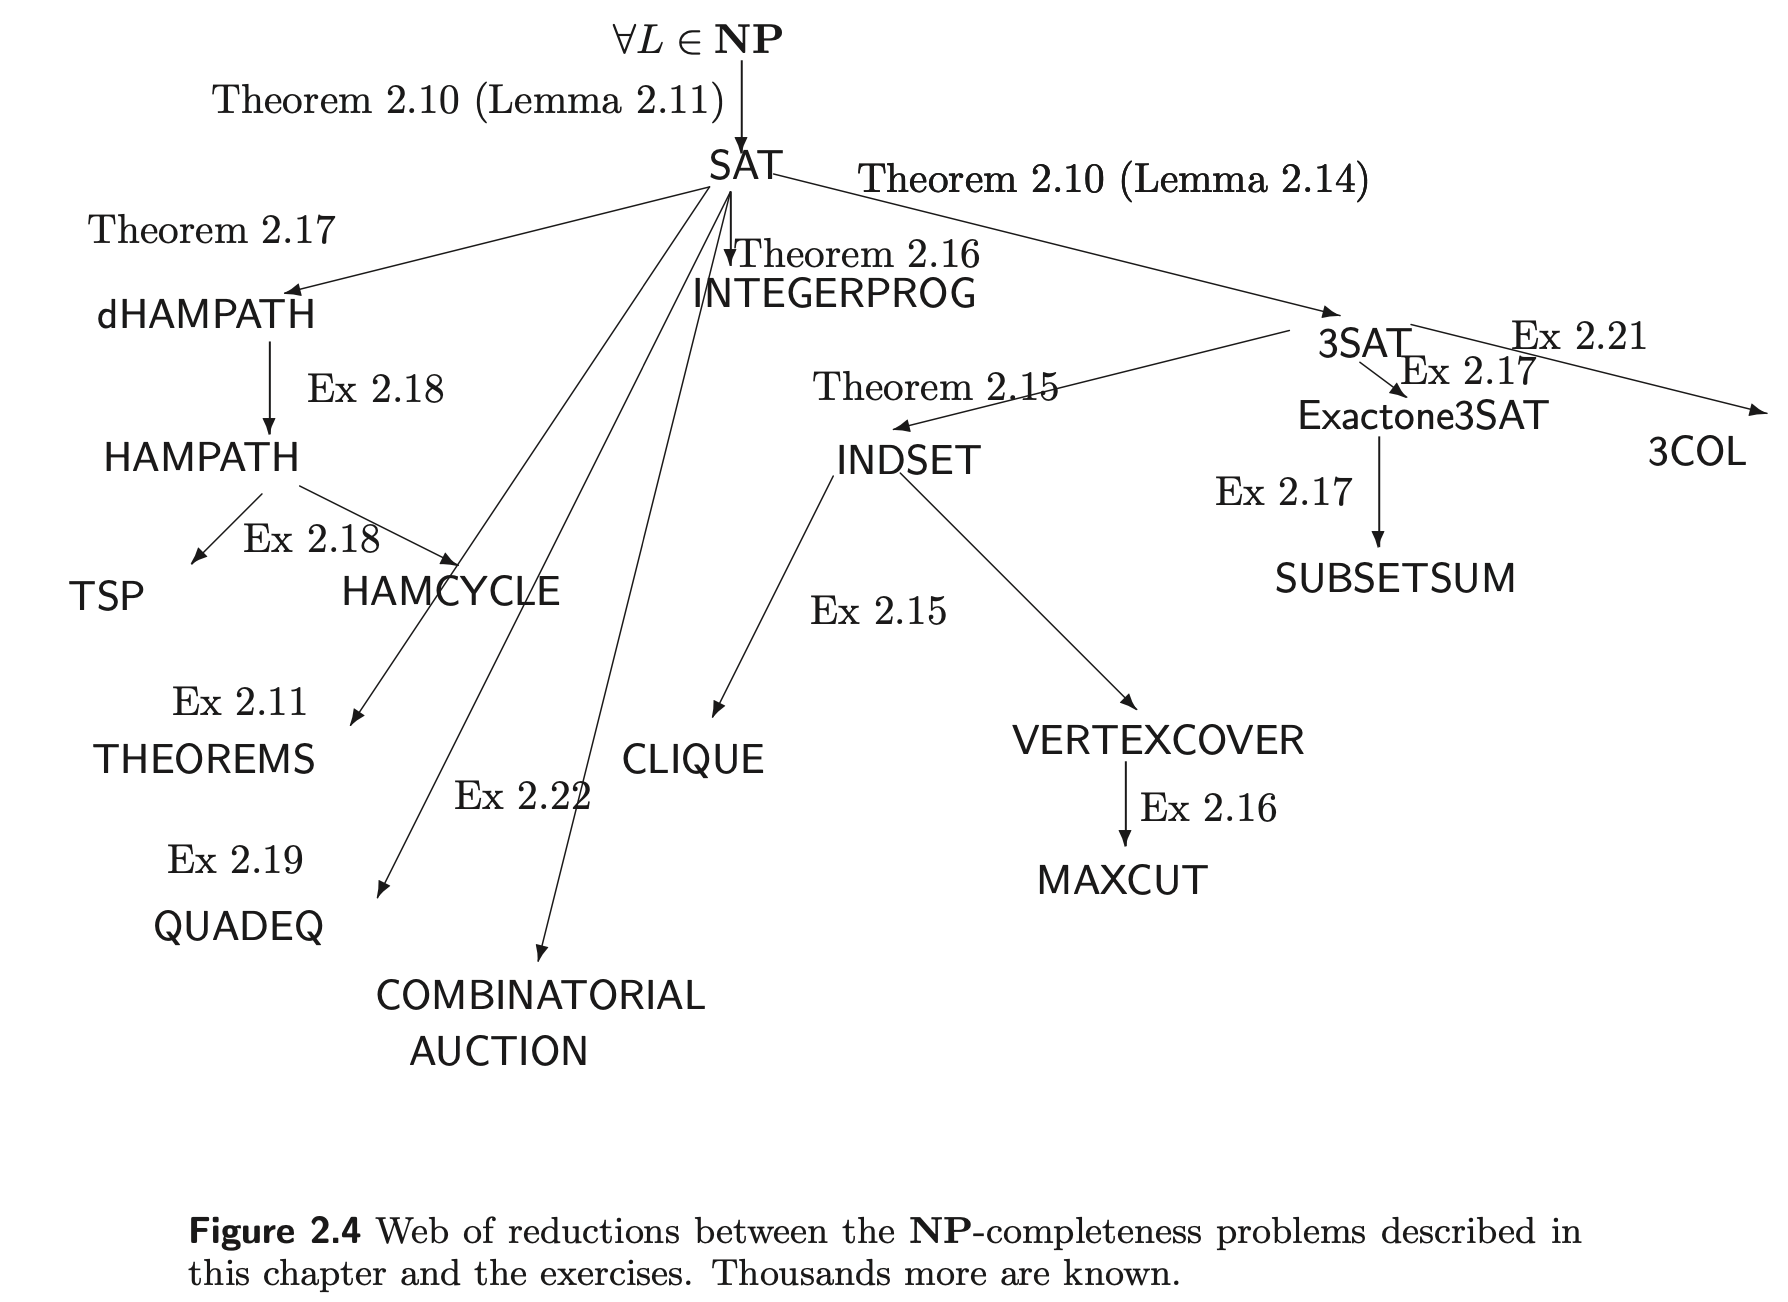
\includegraphics[width=0.95\textwidth]{images/a.png}
        \caption{Another NPC maps}
    \end{figure}
\end{frame}
\begin{frame}
    \frametitle{Definition}
    \begin{definition}[析取范式(CNF)]
        一个布尔表达式$\varphi$, 称$\varphi$为析取范式(CNF), 如果$\varphi$形如:
        \begin{align*}
            \bigwedge_i\left(\bigvee_j v_{i,j}\right)
        \end{align*}
        称$v_{i,j}$为$\varphi$的变量(literal), $(\bigvee_j v_{i,j})$是一个子句(clause).
    \end{definition}
    \pause
    \begin{definition}[SAT and 3SAT]
        $\text{SAT} = \{\text{all satisfiable CNF formulas}\}$ \\
        $\text{3SAT} = \{\text{all satisfiable 3CNF formulas}\}$.
    \end{definition}
\end{frame}
\begin{frame}
    \frametitle{Cook-Levin Theorem}
    \begin{theorem}[Cook-Levin Theorem]
        $\text{3SAT}$是NP-complete的.
    \end{theorem}
    证明: (1) SAT $\in$ NP 是显然的, 考虑证书为一组赋值即可, 验证机只需验证是否可满足.

    (2) SAT 是 NP-hard的. 这个比较困难. 不加证明的给出一个引理.
    \begin{lemma}
        对任意一个布尔函数$f:\{0,1\}^n \rightarrow \{0,1\}$, 可以在$\Theta(2^n)$的时间内构造一个CNF $F$, 使得$f(x) = 1 \iff F(x) = 1$.
    \end{lemma} 
\end{frame}

\subsection{More NPC Problems}
\begin{frame}
    \frametitle{3SAT}
    SAT $\le_p$ 3SAT.
\begin{itemize}
    \item 设$\varphi$是一个CNF公式, 考虑如下规约$f$.
    \item 例如: $(a_1\lor a_2 \lor a_3 \lor a_4) \rightarrow (a_1\lor a_2 \lor z) \land (\bar{z}\lor a_3 \lor a_4)$ 
    \item 一般情况下, 考虑一个有$l$个lieral的子句$(a_1\lor a_2 \lor \cdots \lor a_l)$:
    \begin{align*}
        (a_1\lor a_2 \lor z_1) \land (\bar{z}_1\lor a_3 \lor z_2) \land \cdots \land (\bar{z}_{l-3}\lor a_{l-1}\lor a_l)
    \end{align*}
    总共$l-2$个子句.
\end{itemize}
\end{frame}
\begin{frame}
    \frametitle{MAX-SAT}
    \begin{definition}[MAX-SAT]
        给定一个CNF公式$\varphi$($n$个变量和$m$个子句)和正整数$k$, 如果存在赋值使得$\varphi$中至少有$k$个子句为真, 则$\left\langle \varphi,k\right\rangle \in $MAX-SAT.
    \end{definition}
    SAT $\le_p$ MAX-SAT.
    \begin{itemize}
        \item $\forall \varphi \in$ SAT, 令$k = m$, 则$\left\langle \varphi,k\right\rangle \in$ MAX-SAT.
    \end{itemize}
    MAX-SAT $\in$ NP. 考虑证书为一组赋值即可.
\end{frame}

\begin{frame}
    \frametitle{INDSET}
    \begin{definition}[INDSET]
        给定一个图$G$和正整数$k$, 判定是否存在一个大小为$k$的独立集.
    \end{definition}
    3SAT $\le_p$ INDSET.
    \begin{itemize}
        \item 设$\varphi$是一个3CNF公式(存在$n$个变量和$m$个子句), 构造一个图$G = (V,E)$如下:
        \item $V$: 每个子句$C_i$对于七个点. 这七个点对应7种可能的赋值情况.
        \item $E$: 对应的赋值情况发生冲突, 则在这两点间连边.
    \end{itemize}
\end{frame}

\begin{frame}
    \frametitle{Vertex Cover and CLIQUE}
    \begin{definition}
        \begin{itemize}
            \item \textbf{Vertex Cover}: 给定一个图$G$和正整数$k$, 判定是否存在一个大小不超过$k$的顶点覆盖.
            \item \textbf{CLIQUE}: 给定一个图$G$和正整数$k$, 判定是否存在一个大小不小于$k$的团.
        \end{itemize}
    \end{definition}
    有如下的引理:
    \begin{lemma}
        对任意的无向图$G = (V,E)$和子集$V' \subseteq V$, 下列命题等价:
        \begin{itemize}
            \item $V'$ 是$G$的一个顶点覆盖.
            \item $V-V'$ 是$G$的独立集.
            \item $V - V'$是补图$G_c = (V, E_C)$的团.
        \end{itemize}
    \end{lemma}
\end{frame}

\begin{frame}
    \frametitle{Vertex Cover and CLIQUE(Cont.)}
    INDSET $\le_P$ Vertex Cover.
    \begin{itemize}
        \item $f: \left\langle G,k\right\rangle \rightarrow \left\langle G',k'\right\rangle$, 令$G' = G$, $k' = |V| - k$.
    \end{itemize}
    INDSET $\le_P$ CLIQUE.
    \begin{itemize}
        \item $f: \left\langle G,k\right\rangle \rightarrow \left\langle G',k'\right\rangle $, 令$G' = G_c$, $k' = |V| - k$.
    \end{itemize}
    \begin{figure}
        \centering
        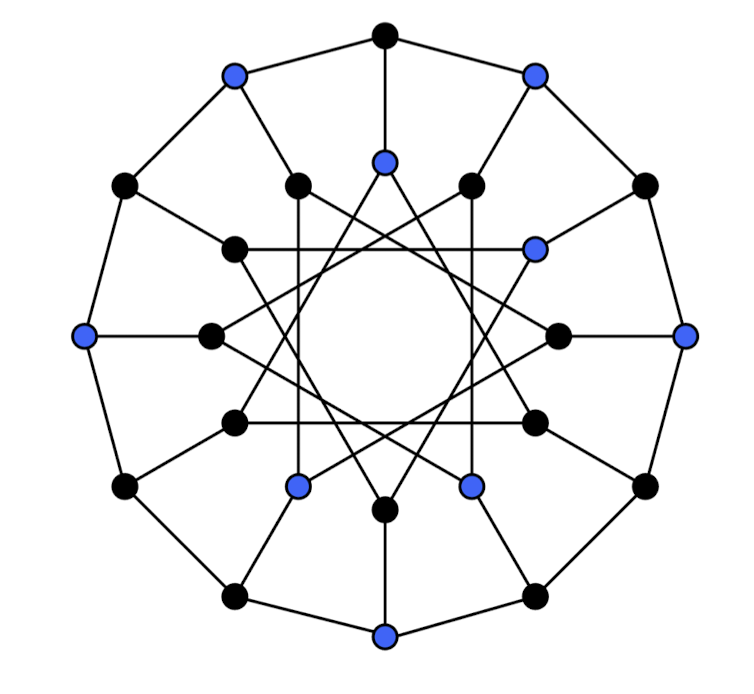
\includegraphics[width=0.5\textwidth]{images/vc.png}
        \caption{Vertex Cover and CLIQUE}
    \end{figure}
\end{frame}

\begin{frame}
    \frametitle{HAMILTONIAN相关问题}
    \begin{definition}
        \begin{itemize}
            \item \textbf{dHAMPATH}: 有向图版本的哈密顿路径.
            \item \textbf{dHAMCYCLE}: 有向图版本的哈密顿回路.
            \item \textbf{uHAMPATH}: 无向图版本的哈密顿路径.
            \item \textbf{uHAMCYCLE}: 无向图版本的哈密顿回路.
        \end{itemize}
    \end{definition}
    下面的证明路径是:
    \begin{align*}
        \text{3SAT} \le_p \text{dHAMPATH} \le_p \text{dHAMCYCLE} \\
        \text{dHAMPATH} \le_p \text{uHAMPATH}.
    \end{align*}
\end{frame}
\begin{frame}
    \frametitle{TSP}
    \begin{definition}[TSP]
        给定一个完全图$G$, 每条边有一个距离$d_{ij}$, 给定正整数$k$, 判定是否存在一个哈密顿回路, 使得总距离不超过$k$.
    \end{definition}
    dHAMCYCLE $\le_p$ TSP.
    \begin{itemize}
        \item 设$G = (V,E), G' = (V',E,)$, $f: \left\langle G\right\rangle \rightarrow \left\langle G', d_{ij}, k\right\rangle$
        \item $V' = V$, 如果$(i,j) \in E$, 则$d_{ij} = 1$, 否则$d_{ij} = +\infty$.
        \item 令$k = |V|$. 那么有$G \in \text{dHAMPATH} \iff \left\langle G', d_{ij}, k\right\rangle \in \text{TSP}$
    \end{itemize}
\end{frame}
\begin{frame}
    \frametitle{Karp's 21 Problems}
    \begin{figure}[H]
        \centering
        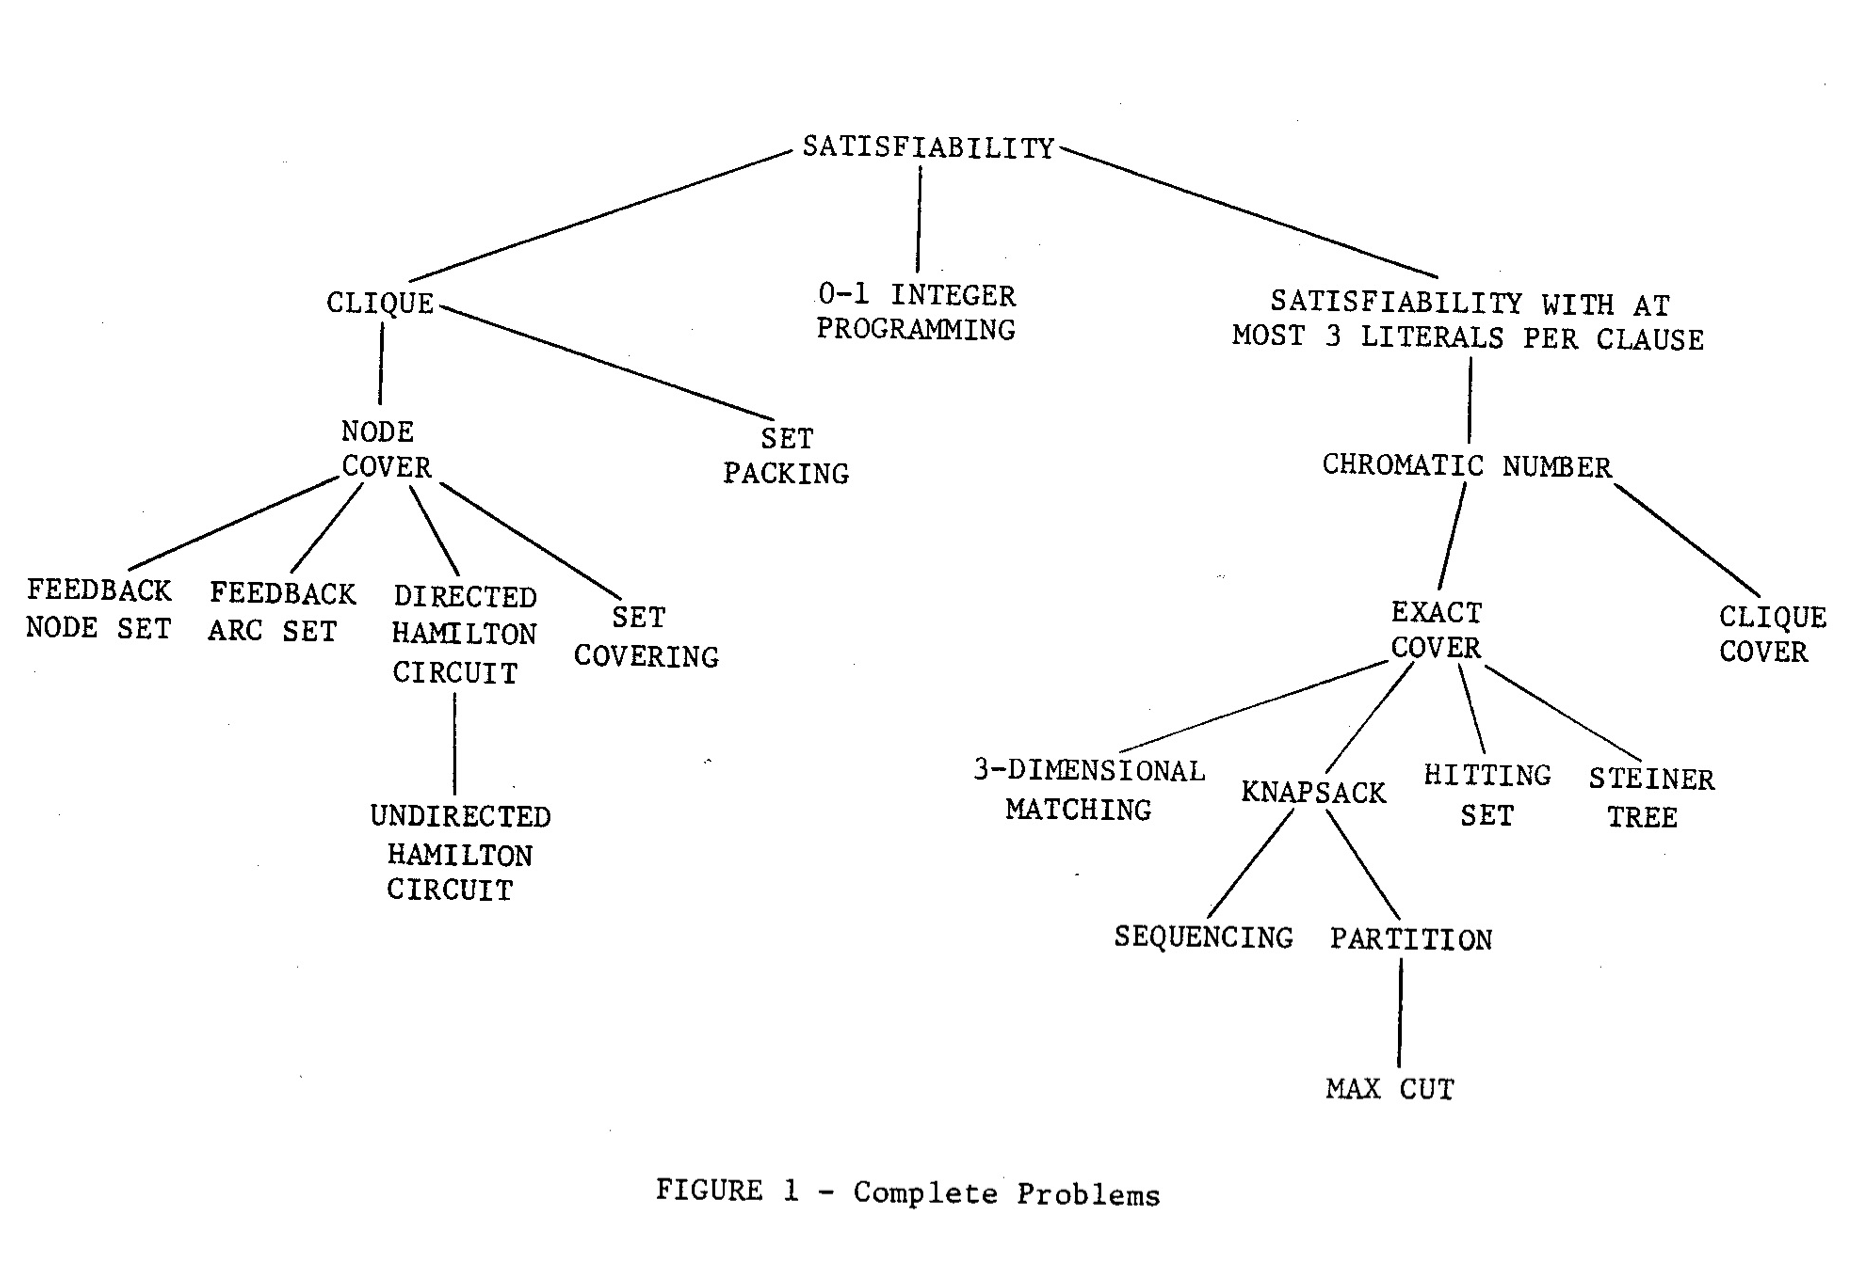
\includegraphics[width=1\textwidth]{images/Karp.png}
        \caption{Karp's 21 Problems}
    \end{figure}
\end{frame}


\end{document}